In this section we apply bandit algorithms on SA-problem and evaluate its performance on synthetic and real datasets. For synthetic example, we consider data transmission over a binary symmetric channel, and for real world examples, we use diabetes (PIMA indiana) and heart disease (Clevland) from UCI dataset. In both datasets attributes/features are associated with costs, where features related to physical observations are cheap and that obtained from medical tests are costly. The experiments are setup as follows:

{\bf Synthetic:} we consider data transmission over two binary symmetric channels (BSCs). Channel $i=1,2$ flips input bit with probability $p_i$ and $p_1\geq p_2$. Transmission over channel $1$ is free and that over channel $2$ costs $ c_2 \in (0,1] $ units per bit. Input bits are generated with uniform probability and we set $p_1=.2$ and $p_2=.1$.

{\bf Datatsets:} we obtain a sensor acquisition setup from the datasets as follows: Two svm classifiers (linear, $C=.01$) are trained for each dataset, one using only cheap features, and the other using all features. These classifiers form sensors of a two stage SAP where classifier trained with cheap features is the first stage and that trained with all features forms the second stage. Cost of each stage is the sum of cost of features used to train that stage multiplied by a scaling factor $\lambda$ (trade-off parameter for accuracy and costs). Specific details for each dataset is given below.  

{\bf PIMA indians diabetes} dataset consists of $768$ instances and has $8$ attributes. The labels identify if the instances are diabetic or not. $6$ of the attributes (age, sex, triceps, etc.) obtained from physical observations are cheap, and $2$ attributes (glucose and insulin) require expensive tests. First sensor of SAP is trained with $6$ cheap attributes and costs \$$6$. Second sensor is trained from all $8$ attributes that cost \$$30$. We set $c_1= 6\lambda, c_2= 30\lambda$ and $c= 24\lambda$.

{\bf Heart disease} dataset consists of $297$ instance (without missing values) and has $13$ attributes. $5$ class labels $(0,1,2,3,4)$ are mapped to binary values by taking value $0$ as `absence' of disease and values $(1,2,3,4)$ as `presence' of disease. First senor of SAP is trained with $7$ attributes which cost  \$$1$ each. Total cost of all attributes is \$$568$. We set $c_1= 7\lambda, c_2= 568\lambda$ and $c= 561\lambda$.

Various error probabilities for synthetic and datasets are listed in Table (\ref{tab:ErrorTable}).  
The probabilities for the datasets are computed on $20 \%$ hold out data. To run the online algorithm, an instance is randomly selected from the dataset in each round and is input to the  algorithm. We repeat the experiments $20$ times and average is shown in (\ref{fig: RegretPlot}) with $95\%$ confidence bounds. The left Figure in \ref{fig: RegretPlot} depicts regret per round vs. cost $c$ for each setup. As seen, regret per round is positive over an interval where it is increasing and then drops to zero sharply. For all $c$ in $[0.1\; 0.26], [0.07\; 0.21], [0.13, \; 0.237]$ for synthetic, diabetes and heart dataset, respectively, the regret per round is positive implying that regret is linear in these regions, and regret per round  sharply falls to zero outside this region implying sublinear regret there. This is in agreement with the weak dominance property. For the BSC setup, regret is plotted on the right of Figure  (\ref{fig: RegretPlot}). As seen, regret is linear for all $c$ in    $[0.1\; 0.26]$ and is sublinear outside this region. 
\begin{figure}
	\begin{minipage}{5cm}
		\small
		\hspace{-1cm}
	\begin{tabular}[c]{c|c|c|c|c } 
		\label{tab:ErrorTable}
	%	\caption{cap:Error statistics}
		dataset & $\gamma_1$ & $\gamma_2$ & $p_{12}$ & $\delta_{12}$\\ \hline 
		BSC & .2 & .1 & .261 & .08\\  \hline
		diabetic & $0.288 $ & $ 0.219$ & $ 0.219$ & 0.075\\  \hline
		heart & $0.305$ & $0.169$ & $0.237$ & 0.051\\  \hline
	\end{tabular}
		\caption{Error statistics}
	\end{minipage}  \hspace{1cm}
	\begin{minipage}{8cm}
		\vspace{-1cm}
		\centering
		\subfigure{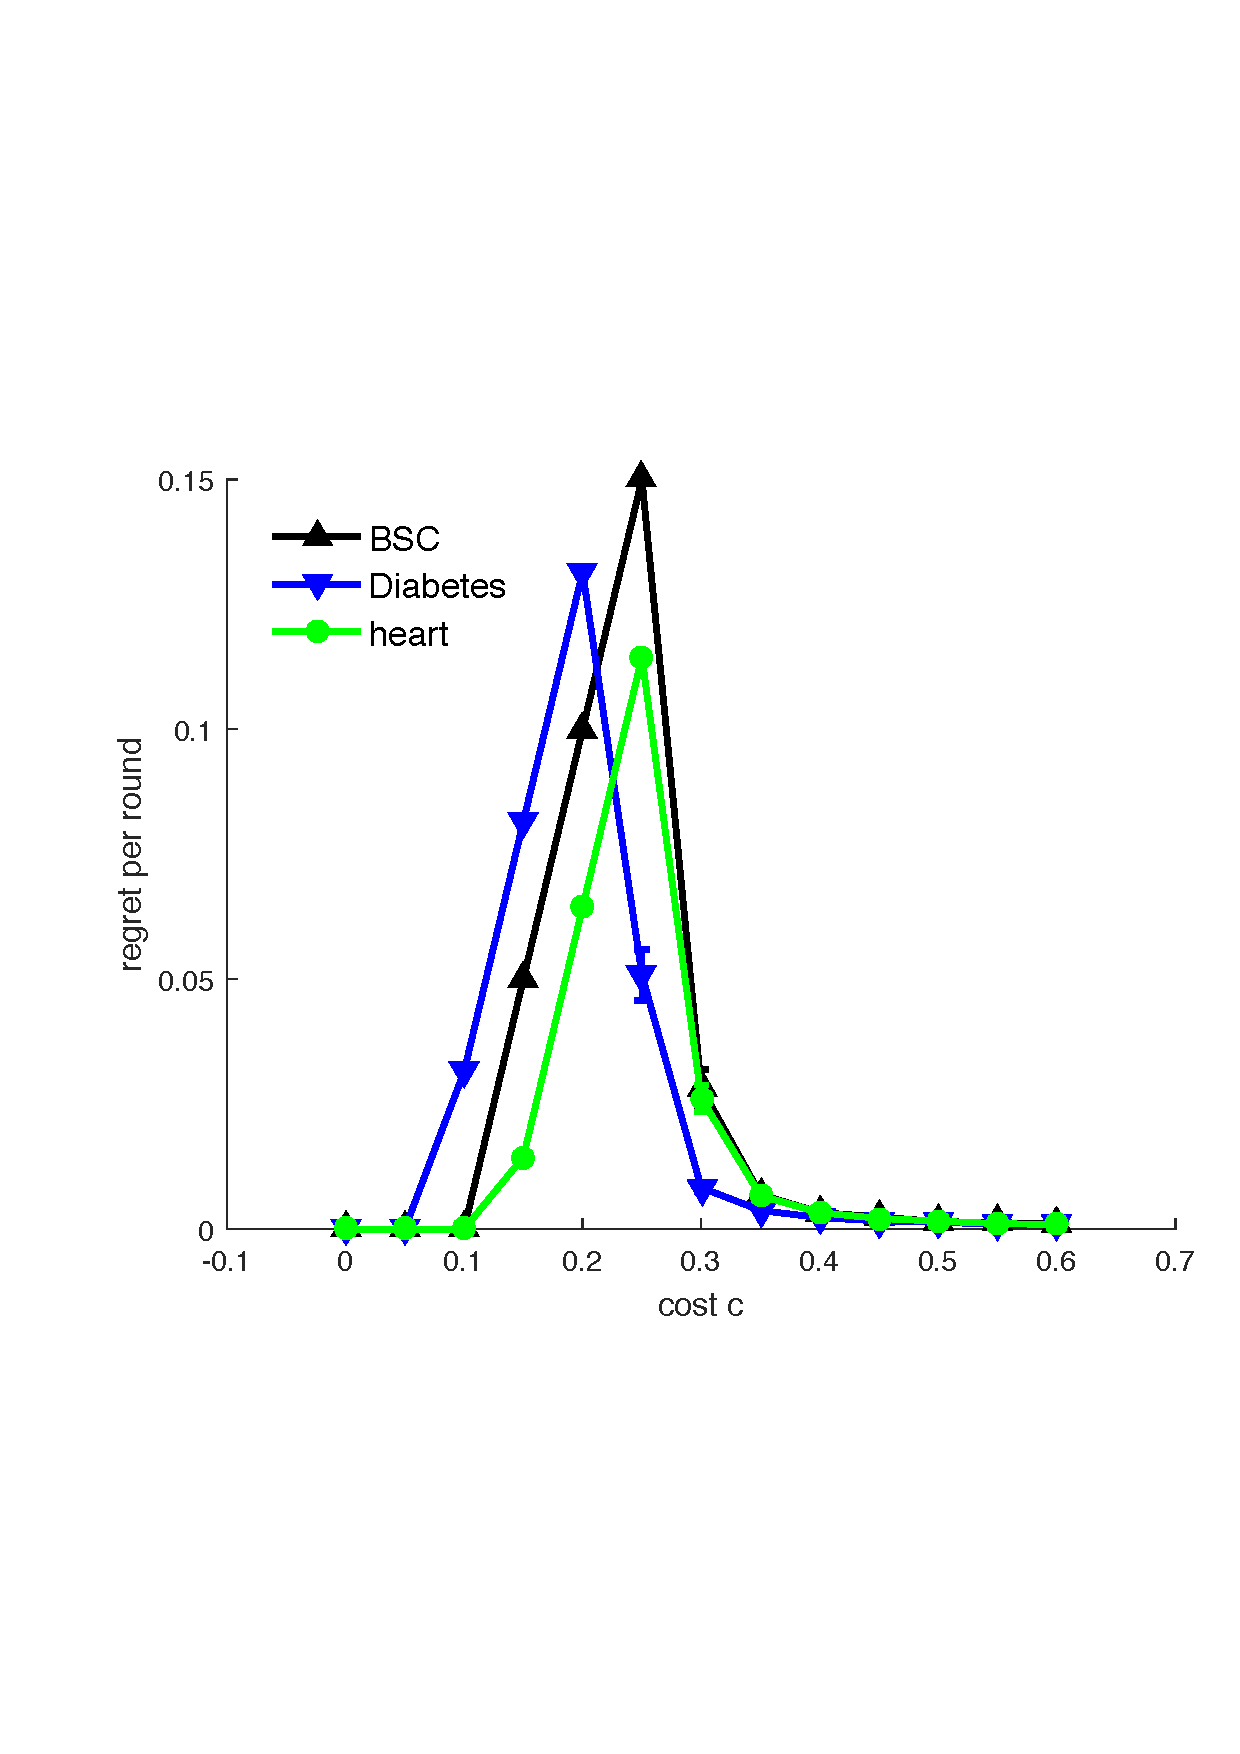
\includegraphics[scale=0.15]{../Simulations/Figures/RegVsCost}}
		\subfigure{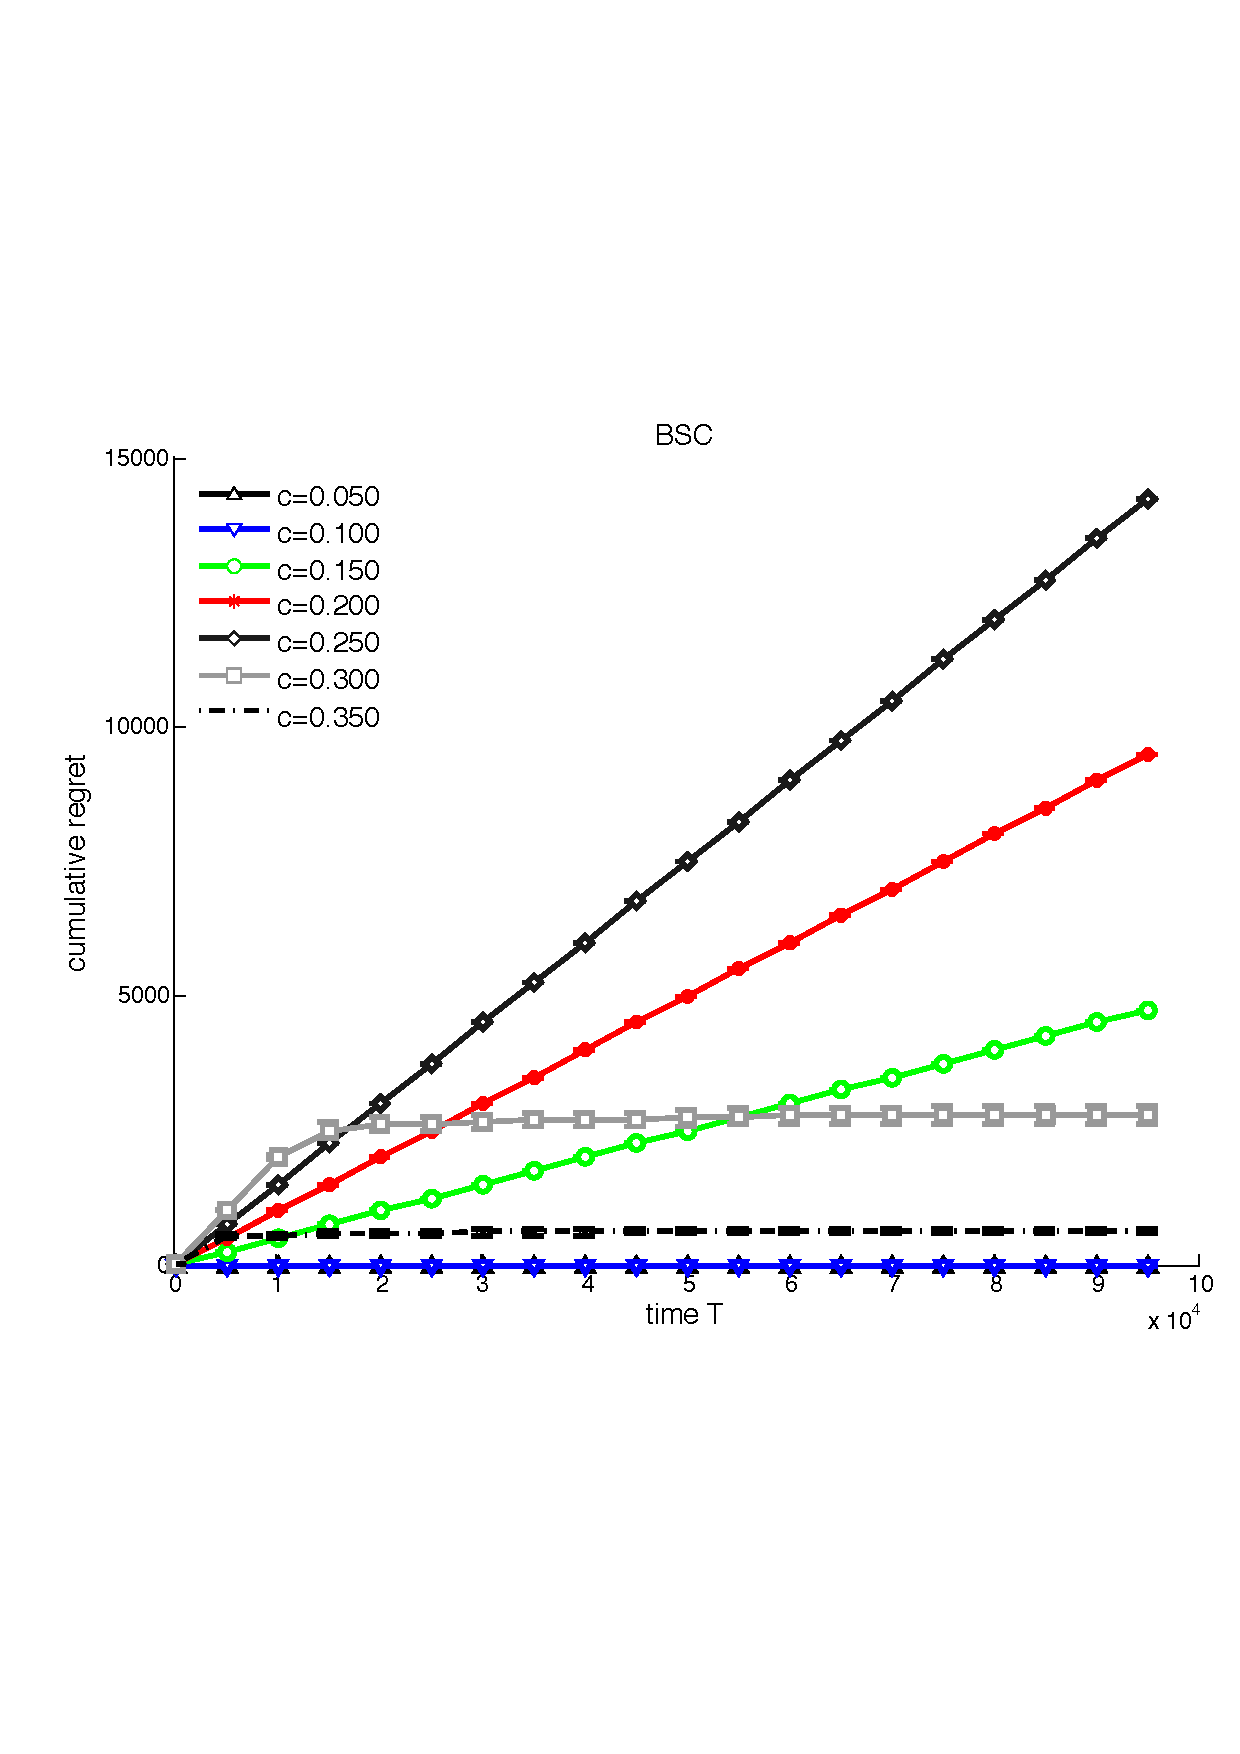
\includegraphics[scale=0.15]{../Simulations/Figures/RegVsTime}}
		\vspace{-1cm}
		\label{fig: RegretPlot}
	\caption{Left side figure plots regret per round against cost for all the datasets. The right side plots regret for different cost in BSC experiment}
	\end{minipage}
	
\end{figure}

